\secnumbersection{PROPUESTA DE SOLUCIÓN}
En la presente sección se realiza una descripción detallada del algoritmo SLAM diseñado para cumplir los objetivos de la memoria, luego se presentará el diseño del algoritmo en conjunto con el pseudocódigo asociado y para finalizar un diagrama para identificar el flujo del mismo.


\subsection{DESCRIPCIÓN}
Tras lo escrito en la sección del marco conceptual y luego explayado en el estado del arte de los algoritmos SLAM, se pueden destacar 3 líneas de investigación de estos algoritmos en los cuales se pueden observar 4 problemas esenciales. En esta memoria se abordará una propuesta de solución para el problema de localización tridimensional en un robot móvil autónomo, es decir, el problema del SLAM 3D agregando un nuevo elemento en la asociación de los datos.

La propuesta del algoritmo SLAM, se basa fuertemente en la investigación realizada por Armin Hornung en \cite{hornung13auro}, en dónde se aborda la problemática desde un punto de vista nuevo y mediante un \textit{framework Open Source}. El framework utiliza la representación de volúmenes mediante octrees \footnote{ La representación volumétrica de octrees propuesta inicialmente en \cite{614315}, plantea la subdivisión recursiva del espacio tridimensional en octantes, creando un árbol con exactamente 8 subnodos y así sucesivamente.}, dicha representación se puede observar en la Figura \ref{fig:octree_tree}.

\begin{figure}[h]
    \centering
    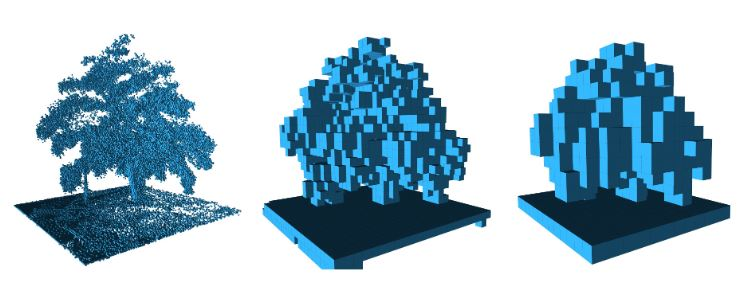
\includegraphics[width=0.8\textwidth]{figures/03propuesta_solucion/octree_mapping.JPG}
    \caption{\label{fig:octree_tree} Representación volumétrica utilizando octree de un árbol} 
    Fuente: \cite{inproceedings}
\end{figure}

EL trabajo desarrollado por Armin Hornung busca resolver el problema a partir de la utilización de LIDARES 3D para obtener dicha representación, lo que si bien aporta en reducir la incertidumbre de la posición, eleva en gran medida el coste económico asociado a dicha solución. Por lo que la propuesta expuesta y desarrollada en esta memoria utiliza la base matemática del algoritmo, sin embargo, se modifica para realizar el mapeo y localización tridimensional a través de una cámara de profundidad y un LIDAR bidimensional para realizar las correcciones necesarias a la información obtenida por la cámara, es decir, mejorar el asociamiento de los datos sin una aumentar en gran medida la incertidumbre del algoritmo a la hora de localizarse en el mapa y de esta manera, plantear un nuevo punto de acción a la problemática del SLAM 3D.

En términos generales, el algoritmo consta con 3 pasos:
\begin{itemize}
    \item Se debe inicializar el nodo maestro de ROS, de tal manera de enlazar correctamente los nodos hijos, establecer los tópicos de comunicación y los tipos de datos a enviar, como también se inicializan los nodos secundarios encargados del control del robot y obtención de datos de los sensores
    \item Se comienza con la obtención de los datos de los sensores, y a los marcadores obtenidos por la cámara se les realiza una corrección de manera que estos coincidan con los datos del LIDAR. Los datos una vez corregidos se guardan en un array multidimensional.
    \item El array multidimensional se procesa con el algoritmo octree recursivamente hasta el nivel 8 \footnote{ Se realizó una estimación del coste computacional asociado a cada nivel y la precisión del mapa generado y se obtuvo que el óptimo está entre el nivel 8 y el nivel 12. Cabe destacar que estos valores son \textbf{solo} para ambientes controlados o de interior.}. Para luego generar la estructura del mapa y transmitirlo en tiempo real.
\end{itemize}

La representación del mapa que el algoritmo genera, corresponde a una mapa probabilístico \footnote{Un mapa probabilístico asocia los datos a una probabilidad de que estén en el lugar indicado, en caso de que la probabilidad sea menor al filtro, entonces dicho dato se muestra como vacío.}. Un ejemplo de este mapa se puede observar en la Figura \ref{fig:mapeo_tridimensional}.

\begin{figure}[H]
    \centering
    \begin{subfigure}[b]{0.40\textwidth}
    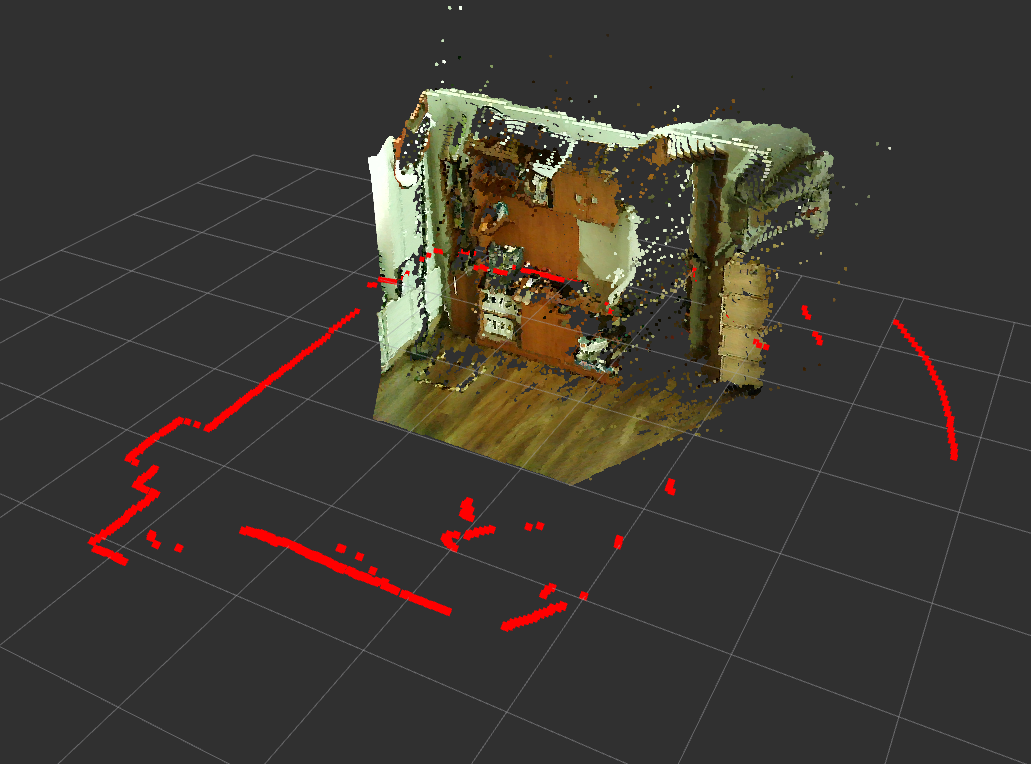
\includegraphics[width=5.5cm, height=4.9cm]{figures/03propuesta_solucion/slam_normal.png}
    \caption{Entorno mapeado utilizando la cámara de profundidad y LIDAR}
    \label{fig:gmapping_sim}
    \end{subfigure}
    \hspace{5mm}
    \begin{subfigure}[b]{0.40\textwidth}
        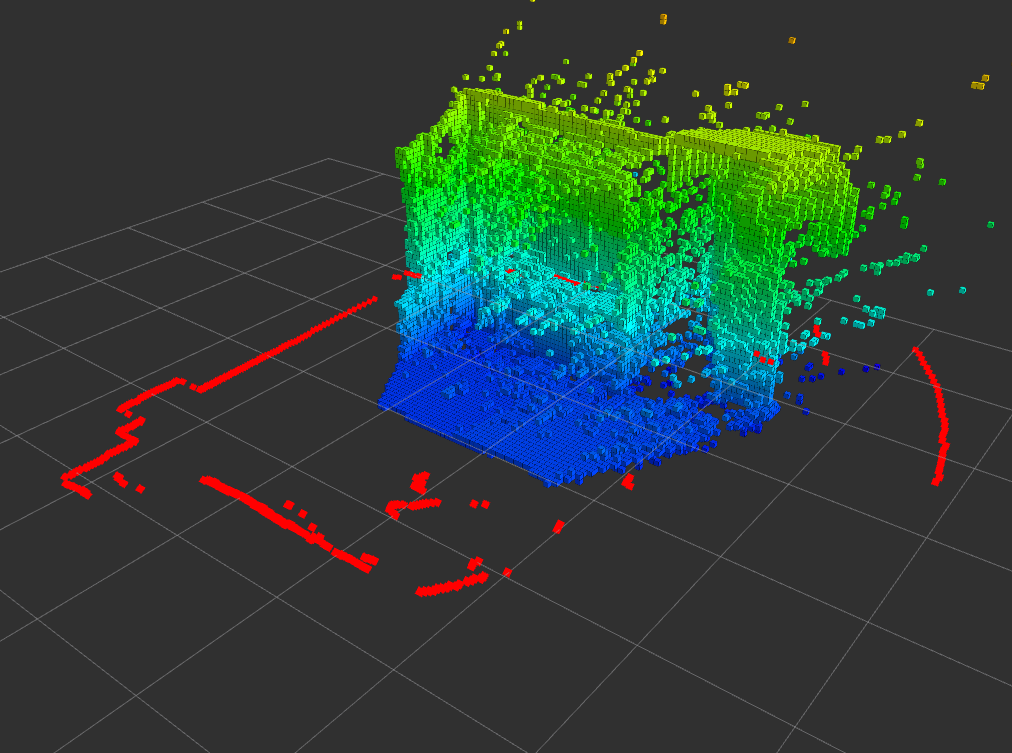
\includegraphics[width=5.5cm, height=4.9cm]{figures/03propuesta_solucion/slam_octree.png}
    \caption{Array multidimensional asociado a los datos obtenidos.}
    \label{fig:gmapping_map}
    \end{subfigure}
    \caption{Proceso de obtención de datos y generación del mapa tridimensional}
    Fuente: Fabricación propia
    \label{fig:mapeo_tridimensional}
\end{figure}


\newpage
\subsection{DISEÑO DEL ALGORITMO}

A continuación se muestra el pseudocódigo del algoritmo propuesto, el que se puede apreciar en el Algoritmo \ref{alg:Algoritmo 3DSLAM propuesto}. El algoritmo utiliza los datos de los diversos sensores para construir el mapa en dos dimensiones, el mapa tridimensional, obtener la orientación y localizarse dentro del mapa. Además se le debe entregar una resolución correspondiente y una precisión para la construcción tridimensional del mapa y finalmente una posición objetivo donde el robot debe ir.

\subsubsection{PSEUDOCÓDIGO}

\begin{algorithm}[H]
\centering
    \begin{algorithmic}[1]
        \Require $C_{d}$, $L_{d}$, $I_{d}$, $E_{d}$, data from sensors
        \Require $N = \{N_i, N_{i+1}, ...\}$, nodes for every sensor
        \Require $R$, resolution of the map
        \Require $A$, accuracy of the algorithm
        \Require $P_{f}$, final position
        \vspace{1mm}
        \hline
        \vspace{1mm}
        \State $A_{m}(R)$, $3DMap$, $2DMap  \leftarrow \emptyset$
        \State $P_a \leftarrow (0,0,0)$
        \ForAll{$N_i \in N$}
            \State initializeNode($N_i$)
        \EndFor
        \While{$Rospy \And P_a \neq P_f$}
            \State $P_{a} \leftarrow $ AMCL($3DMap$)
            \ForAll{$c_i \in C_d \And l_i \in L_d$}
                \State $2DMap  \leftarrow$ writeGridCell($l_{i}$, $2DMap$)
                \State $c_i \leftarrow$ correctionAlgorithm($c_i$, $l_i$) 
                \If {$c_i \notin A_{m}$} 
                    \State $A_{m} \leftarrow c_i$
               \EndIf
            \EndFor
            \State $3DMap \leftarrow$ octreeCodification($A_{m}, A$) 
            \State rvisualization($3DMap$, $2DMap$)
            \If{$P_a \neq P_f$}
                \State driveToGoal($3DMap$, $I_d$, $E_{d}$)
                \State updateStatusRobot()
            \Else
                \State \Return $GOAL$
            \EndIf
        \EndWhile
    \vspace{1mm}
    \hline
    \vspace{1mm}
    \end{algorithmic}
\caption{Pseudocódigo algoritmo 3D SLAM propuesto}
Fuente: Fabricación propia
\label{alg:Algoritmo 3DSLAM propuesto}
\end{algorithm}

\subsubsection{DIAGRAMA DE FLUJO DEL ALGORITMO}

A continuación se presenta el diagrama de flujo del algoritmo propuesto. En el diagrama, el cual se puede apreciar en la Figura \ref{fig:slam_3d_proposal_flujo}, se destacan 4 secciones definidas por 4 colores, cada una de estas secciones tiene tareas específicas las que se describen bajo el siguiente contexto: En color \textbf{verde} se indican los parámetros modificables, en color \textbf{naranjo} se demarcar los datos provenientes de los diversos sensores requeridos para el correcto funcionamiento del algoritmo, en color \textbf{morado} se indica el ciclo principal del algoritmo, es decir, el proceso de adquisición de datos, parametrización, filtrado y construcción del mapa y finalmente en \textbf{azul} el output del algoritmo el cual indica si se llegó al objetivo o no.

\begin{figure}[h]
    \centering
    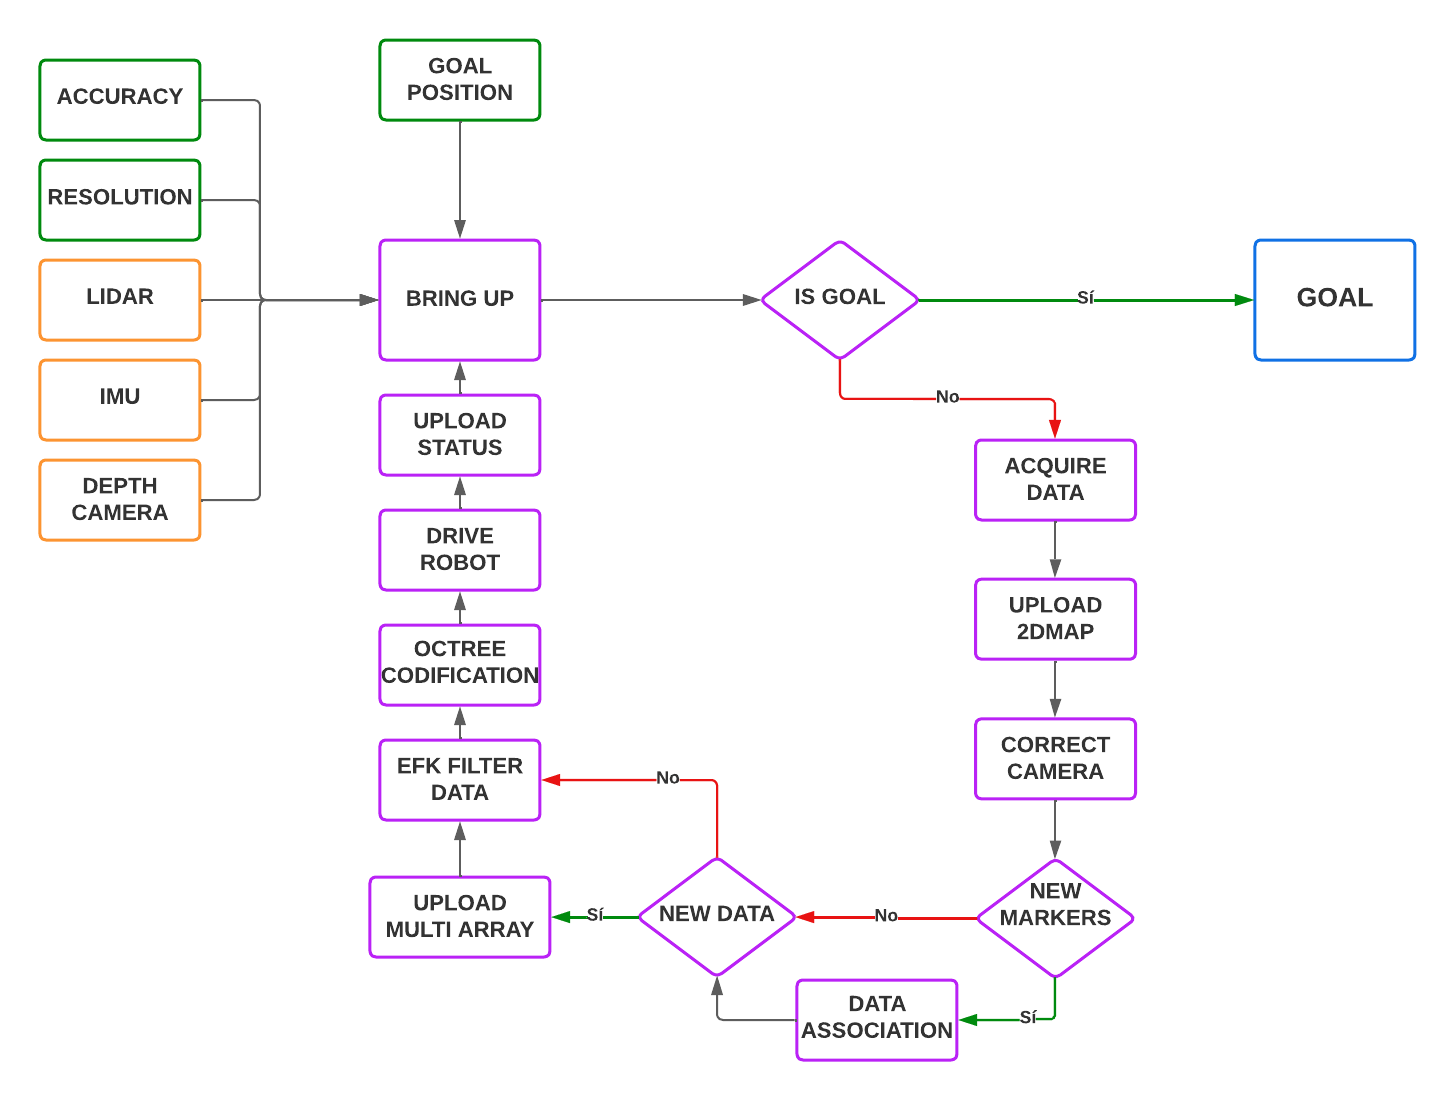
\includegraphics[width=0.8\textwidth]{figures/03propuesta_solucion/slam_3d_proposal.png}
    \caption{\label{fig:slam_3d_proposal_flujo} Diagrama de flujo del algoritmo propuesto} 
    Fuente: Fabricación propia
\end{figure}

Como se dijo anteriormente en el área central con color morado, se destaca el ciclo principal del algoritmo. En este, ocurre lo esencial para producir el SLAM 3D, es decir, se obtienen y procesan los datos provenientes de los sensores y los propios parámetros del algoritmo, se realiza la corrección de los datos de la cámara para que coincidan con los del LIDAR y se realiza un filtrado en los marcadores para diferenciar si el dato ingresado es nuevo o es un dato ya leído. Finalmente el algoritmo produce un filtrado EFK a los datos guardados en un array multidimensional para proceder con la codificación en octree, realizar el movimiento del robot y actualizar su status.




\begin{comment}

Se debe desarrollar la solución propuesta. Los subcapítulos por poner aquí son propios del autor. Se sugiere mencionar metodología usada. Es conveniente incorporar figuras y tablas para aclarar la solución, que deben indicar el número de la figura, su nombre y su autor o fuente (si las diseñas tú, la fuente es ``Elaboración propia''). Ver ejemplos en esta página y en la siguiente.

Cabe mencionar que aquí está la esencia del trabajo en lo que se refiere al aporte creativo del memorista, es el momento de demostrar que usted es un destacado profesional que creó, diseñó y/o llevó a cabo la solución propuesta.
\end{comment}